\documentclass[10pt,a4paper,oneside]{article}
\usepackage[utf8]{inputenc}
\usepackage[T1]{fontenc}
\usepackage{newpxtext}
\usepackage[scaled=0.88]{sourcecodepro}
\usepackage{microtype}
\usepackage[a4paper,top=19mm,bottom=19mm,left=20mm,right=20mm,headheight=16pt,footskip=10mm]{geometry}
\usepackage[dvipsnames,table]{xcolor}
\usepackage{amssymb}
\usepackage{graphicx}
\usepackage{booktabs,tabularx,array}
\usepackage{enumitem}
\usepackage{listings}
\usepackage{tikz}
\usetikzlibrary{arrows.meta,positioning}
\usepackage{titlesec}
\usepackage{fancyhdr}
\usepackage{hyperref}
\definecolor{politoNavy}{RGB}{0,45,98}
\definecolor{steelBlue}{RGB}{35,100,160}
\definecolor{skyBlue}{RGB}{230,240,250}
\definecolor{bodyGray}{RGB}{80,85,90}
\definecolor{codeBg}{RGB}{248,249,251}
\definecolor{codeFrame}{RGB}{220,225,230}
\hypersetup{colorlinks=true,linkcolor=politoNavy,urlcolor=steelBlue,pdftitle={Laboratory 05 complete solution},pdfauthor={Politecnico di Torino}}
\newcommand{\labSolutionTitle}{Laboratory 05: Quantization and Low-Rank Adaptation}
\newcommand{\labSolutionSubtitle}{Complete notebook-aligned solution}
\titleformat{\section}{\normalfont\sffamily\Large\bfseries\color{politoNavy}}{\thesection}{0.8em}{}
\titleformat{\subsection}{\normalfont\sffamily\large\bfseries\color{steelBlue}}{\thesubsection}{0.8em}{}
\pagestyle{fancy}\fancyhf{}
\fancyhead[L]{\small\sffamily\color{bodyGray}\nouppercase{\rightmark}}
\fancyhead[R]{\small\sffamily\bfseries\thepage}
\renewcommand{\headrulewidth}{0.4pt}
\fancypagestyle{plain}{\fancyhf{}\fancyfoot[C]{\small\sffamily\thepage}\renewcommand{\headrulewidth}{0pt}}
\lstdefinestyle{studycode}{language=Python,basicstyle=\fontsize{7.4}{8.8}\ttfamily,keywordstyle=\bfseries\color{politoNavy},commentstyle=\itshape\color{bodyGray},stringstyle=\color{ForestGreen},numbers=left,numberstyle=\tiny\color{bodyGray},numbersep=6pt,tabsize=4,showstringspaces=false,breaklines=true,breakatwhitespace=false,columns=fullflexible,keepspaces=true,frame=single,rulecolor=\color{codeFrame},backgroundcolor=\color{codeBg},literate={█}{{\ensuremath{\blacksquare}}}1 {▎}{{|}}1 {▋}{{|}}1 {—}{{---}}1 {’}{{'}}1}
\lstdefinestyle{terminalOutput}{basicstyle=\fontsize{7.2}{8.5}\ttfamily,breaklines=true,breakatwhitespace=false,columns=fullflexible,keepspaces=true,showstringspaces=false,frame=single,rulecolor=\color{codeFrame},backgroundcolor=\color{codeBg},literate={█}{{\ensuremath{\blacksquare}}}1 {▎}{{|}}1 {▋}{{|}}1 {—}{{---}}1 {’}{{'}}1}
\lstset{style=studycode}
\setlist{nosep,leftmargin=1.5em}
\begin{document}
\begin{titlepage}
\centering
\vspace*{8mm}

\includegraphics[width=0.30\textwidth]{../../figures/branding/polito_logo.pdf}\par
\vspace{8mm}
{\large\scshape Politecnico di Torino\par}
\vspace{2mm}
{\normalsize Master of Science in Computer Engineering\par}
{\small Department of Control and Computer Engineering (DAUIN)\par}
\vspace{12mm}
\rule{\linewidth}{1.2pt}\par\vspace{5mm}
{\Huge\bfseries\color{politoNavy}Large Language Models\\[2mm]for Software Engineering\par}
\vspace{6mm}
{\Large\bfseries\color{steelBlue}\labSolutionTitle\par}
\vspace{3mm}
{\large\labSolutionSubtitle\par}
\vspace{5mm}
\rule{\linewidth}{1.2pt}\par
\vfill
\begin{minipage}[t]{0.47\textwidth}
\raggedright
\emph{Course Instructor}\par
\textbf{Prof.~Flavio Giobergia}\par\vspace{5mm}
\emph{Laboratory Assistant}\par
\textbf{Claudio Savelli}
\end{minipage}\hfill
\begin{minipage}[t]{0.47\textwidth}
\raggedleft
\emph{Prepared by}\par
\textbf{Nicola Beccaceci}\par\vspace{5mm}
\emph{Academic Year}\par
\textbf{2026/2027}
\end{minipage}
\vfill
{\small\sffamily\color{bodyGray}Politecnico di Torino\quad|\quad Torino, Italy\par}
\end{titlepage}

\tableofcontents
\clearpage
\documentclass[../labs.tex]{subfiles}
egin{document}

\section[Quantization]{Quantization: from low-bit arithmetic to Llama inference}

\label{sec:lab05-quant}

This exercise first makes low-bit arithmetic visible on a small matrix and vector, where symmetric and asymmetric quantization can be compared directly. It then applies post-training quantization to Llama 3.2 1B, measuring serialized size and a fixed CPU generation workload across float32, PyTorch int8, and BitsAndBytes int4. The toy example isolates rounding, zero points, and accumulation overflow; the model experiment shows how these ideas behave in a real decoder-only network.

\begin{figure}[htbp]
\centering
\resizebox{\linewidth}{!}{%
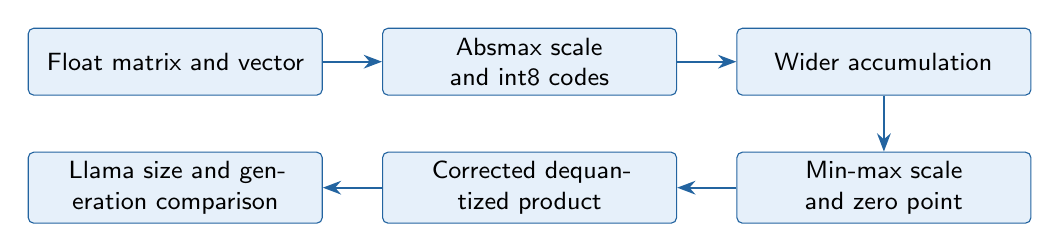
\begin{tikzpicture}[>=Stealth,stage/.style={draw=steelBlue,fill=skyBlue,rounded corners=2pt,align=center,text width=3.5cm,minimum height=.85cm,font=\small\sffamily}]
\node[stage] (a) at (0cm,0cm) {Float matrix and vector};
\node[stage] (b) at (4.5cm,0cm) {Absmax scale and int8 codes};
\node[stage] (c) at (9cm,0cm) {Wider accumulation};
\node[stage] (d) at (9cm,-1.6cm) {Min-max scale and zero point};
\node[stage] (e) at (4.5cm,-1.6cm) {Corrected dequantized product};
\node[stage] (f) at (0cm,-1.6cm) {Llama size and generation comparison};
\draw[->,thick,steelBlue] (a) -- (b);
\draw[->,thick,steelBlue] (b) -- (c);
\draw[->,thick,steelBlue] (c) -- (d);
\draw[->,thick,steelBlue] (d) -- (e);
\draw[->,thick,steelBlue] (e) -- (f);
\end{tikzpicture}%
}
\caption{The exercise pipeline, from input to checked result.}
\end{figure}

\subsection{Absmax quantization and accumulation}

\smallskip
\noindent We start with a fixed seed and two small tensors: a 3 by 5 weight matrix and a length-five input vector. Setting one coordinate in each to zero makes it possible to observe how the two quantizers treat zero.
\label{res:lab05-quant-0003}
% coverage-cell: LABS/lab05/text-01-quantization.ipynb cell=3 source_sha256=36d8465a225041e4137948f7d288391a1f9f36d6ec456b55ece09ba07798521d
\begin{lstlisting}[style=studycode]
import torch

torch.random.manual_seed(0)

n_rows = 3
n_cols = 5

# TODO: Create two random tensors, W (of shape n_rows, n_cols) and x (of shape n_cols)
W = torch.randn(n_rows, n_cols)
x = torch.randn(n_cols)

W[0,0] = 0
x[0] = 0
\end{lstlisting}
\par\smallskip
These tensors are the common reference for the unquantized product and both quantization schemes. Their small dimensions keep the integer arithmetic inspectable.

\smallskip
\noindent Before changing precision, this product records the reference output of the original matrix and vector. Every later reconstruction is compared with this value.
\label{res:lab05-quant-0006}
% coverage-cell: LABS/lab05/text-01-quantization.ipynb cell=6 source_sha256=1f4bacc662bf07b1d5372d3f59e743e82b87f396e5466e15ac548647347ef0e4
\begin{lstlisting}[style=studycode]
out = W @ x
print(out)
\end{lstlisting}
\par\smallskip
% coverage-output: LABS/lab05/text-01-quantization.ipynb cell=6 output=0 source_sha256=1f4bacc662bf07b1d5372d3f59e743e82b87f396e5466e15ac548647347ef0e4 payload_sha256=6353ba4ad5c3355d042a7ef79a71bbcc3f3c225d18991264dd529ca9c613118e artifact=study_guide/execution_artifacts/lab05/lab05/text-01-quantization_cell_0006_1f4bacc662bf_output_0.txt
\label{out:lab05-quant-0006-00}
\lstinputlisting[style=terminalOutput]{../../execution_artifacts/lab05/lab05/text-01-quantization_cell_0006_1f4bacc662bf_output_0.txt}
The floating-point result is the numerical target for the quantized calculations that follow.

\smallskip
\noindent This helper implements symmetric absmax quantization. Its scale maps the largest magnitude to 127, rounding maps values to integer levels, and clamping keeps them in the symmetric range from -127 to 127. The zero-range guard makes an all-zero tensor safe to quantize.
\label{res:lab05-quant-0008}
% coverage-cell: LABS/lab05/text-01-quantization.ipynb cell=8 source_sha256=8c7d867fc3092e6060e1083236561c150562e008a487e91817552beaf6d68b50
\begin{lstlisting}[style=studycode]
def absmax_quantize(W):
    # NOTE: we assume that we always map to 8-bit integers

    # TODO: find the scale factor that maps the maximum absolute value in W to the maximum value of int8
    max_value = W.abs().max()
    scale = torch.where(max_value > 0, max_value / 127, torch.ones_like(max_value)) # how "long" the step between any two int8 values is

    # TODO: quantize W using the scale factor (hint: remember to round to the nearest integer and convert to int8)
    W_q = torch.round(W / scale).clamp(-127, 127).to(torch.int8)
    return W_q, scale
\end{lstlisting}
\par\smallskip
The function returns both integer codes and the scale needed to recover approximate floating-point values.

\smallskip
\noindent Quantization is useful only if the integer representation can be interpreted again. This inverse helper converts the codes to float and multiplies by their saved scale.
\label{res:lab05-quant-0010}
% coverage-cell: LABS/lab05/text-01-quantization.ipynb cell=10 source_sha256=a6b840a526c66e13538d8eb87bd63f2b9e18ea000c890372ac2561a0dd523dbe
\begin{lstlisting}[style=studycode]
def absmax_dequantize(W_q, scale):
    # TODO: dequantize W_q using the scale factor
    dequantized_W = W_q.to(torch.float32) * scale
    return dequantized_W
\end{lstlisting}
\par\smallskip
The original scale is required downstream; without it the integer codes do not retain the magnitude of the source tensor.

\smallskip
\noindent We now apply the same symmetric scheme independently to the matrix and vector. Independent scales use each operand's available integer range effectively.
\label{res:lab05-quant-0012}
% coverage-cell: LABS/lab05/text-01-quantization.ipynb cell=12 source_sha256=2571a85a736ce0fe9697c2b88713c40564459a6a0f63d1b5f3bc4e7934e6823c
\begin{lstlisting}[style=studycode]
W_q, scale_W = absmax_quantize(W)
x_q, scale_x = absmax_quantize(x)
\end{lstlisting}
\par\smallskip
The resulting integer tensors and separate scales feed the reconstruction checks and integer dot product.

\smallskip
\noindent This comparison examines the matrix codes, the original weights, and the dequantized approximation. The mean absolute difference condenses coordinate-wise rounding error into one diagnostic.
\label{res:lab05-quant-0013}
% coverage-cell: LABS/lab05/text-01-quantization.ipynb cell=13 source_sha256=f78cda457b8df435ce3033bc8e83502f51d5cd14867f356df2e94e90b44007ad
\begin{lstlisting}[style=studycode]
print(W_q)
print(W)

#TODO: dequantize W_q and check how close it is to the original W
W_deq = absmax_dequantize(W_q, scale_W)
print(W_deq)
W_diff = (W - W_deq).abs().mean()
print(W_diff)
\end{lstlisting}
\par\smallskip
% coverage-output: LABS/lab05/text-01-quantization.ipynb cell=13 output=0 source_sha256=f78cda457b8df435ce3033bc8e83502f51d5cd14867f356df2e94e90b44007ad payload_sha256=9e6c07b77300ffa843cbc68e92c0469ce63086baab6e7151d4c326d37b121950 artifact=study_guide/execution_artifacts/lab05/lab05/text-01-quantization_cell_0013_f78cda457b8d_output_0.txt
\label{out:lab05-quant-0013-00}
\lstinputlisting[style=terminalOutput]{../../execution_artifacts/lab05/lab05/text-01-quantization_cell_0013_f78cda457b8d_output_0.txt}
The reconstructed matrix stays close to the original and preserves the deliberately zero entry. The small nonzero mean error is quantization loss, not a change to the original tensor.

\smallskip
\noindent The same round trip is checked for the input vector, using its own scale. This separates weight error from activation error.
\label{res:lab05-quant-0014}
% coverage-cell: LABS/lab05/text-01-quantization.ipynb cell=14 source_sha256=09bbfce39abaafce8a1c91c90a8dd7fc60fbfc80a62d4511a8c8d51ab9aeda8f
\begin{lstlisting}[style=studycode]
print(x_q)
print(x)

# TODO: dequantize x_q and check how close it is to the original x
x_deq = absmax_dequantize(x_q, scale_x)
print(x_deq)
x_diff = (x - x_deq).abs().mean()
print(x_diff)
\end{lstlisting}
\par\smallskip
% coverage-output: LABS/lab05/text-01-quantization.ipynb cell=14 output=0 source_sha256=09bbfce39abaafce8a1c91c90a8dd7fc60fbfc80a62d4511a8c8d51ab9aeda8f payload_sha256=f49a08afcc71d326604ce61ef1f68c8e0bb4e4f644d166c1306542656ae93f01 artifact=study_guide/execution_artifacts/lab05/lab05/text-01-quantization_cell_0014_09bbfce39aba_output_0.txt
\label{out:lab05-quant-0014-00}
\lstinputlisting[style=terminalOutput]{../../execution_artifacts/lab05/lab05/text-01-quantization_cell_0014_09bbfce39aba_output_0.txt}
The vector reconstruction also preserves zero; its mean absolute error is reported independently from the matrix's.

\smallskip
\noindent This is the tempting low-precision computation: multiply the quantized matrix and vector while they are still int8. It exposes a hardware arithmetic issue separate from the rounding errors measured above.
\label{res:lab05-quant-0016}
% coverage-cell: LABS/lab05/text-01-quantization.ipynb cell=16 source_sha256=fe70f75003c82158d2218d9a4e23820576157618d2a5dc7ed47440c6f559318e
\begin{lstlisting}[style=studycode]
# TODO: perform the matrix multiplication using the quantized values
product = W_q @ x_q 
print(product)
\end{lstlisting}
\par\smallskip
% coverage-output: LABS/lab05/text-01-quantization.ipynb cell=16 output=0 source_sha256=fe70f75003c82158d2218d9a4e23820576157618d2a5dc7ed47440c6f559318e payload_sha256=8dc5706b0bd037f20a8dbc3f0373d75dc4abe9b289c059874e62180cb27f532e artifact=study_guide/execution_artifacts/lab05/lab05/text-01-quantization_cell_0016_fe70f75003c8_output_0.txt
\label{out:lab05-quant-0016-00}
\lstinputlisting[style=terminalOutput]{../../execution_artifacts/lab05/lab05/text-01-quantization_cell_0016_fe70f75003c8_output_0.txt}
The displayed result has wrapped values because the dot products exceed the int8 range. Quantized operands therefore need a wider accumulator even when their storage uses eight bits.

\smallskip
\noindent Inspecting the first matrix row and the vector lets us verify one dot product by hand and compare it with the wrapped result.
\label{res:lab05-quant-0018}
% coverage-cell: LABS/lab05/text-01-quantization.ipynb cell=18 source_sha256=40eae42eb16ae6379677517a1fb68a6812f53d6063e3f5504be8bf79fa7240ad
\begin{lstlisting}[style=studycode]
W_q[0], x_q
\end{lstlisting}
\par\smallskip
% coverage-output: LABS/lab05/text-01-quantization.ipynb cell=18 output=0 source_sha256=40eae42eb16ae6379677517a1fb68a6812f53d6063e3f5504be8bf79fa7240ad payload_sha256=d4b17d2e128030a8c98d248b1cf3e897c2cc3248cfd5db3a151e1fd1efe5c597 artifact=study_guide/execution_artifacts/lab05/lab05/text-01-quantization_cell_0018_40eae42eb16a_output_0.txt
\label{out:lab05-quant-0018-00}
\lstinputlisting[style=terminalOutput]{../../execution_artifacts/lab05/lab05/text-01-quantization_cell_0018_40eae42eb16a_output_0.txt}
The integer operands are individually representable in int8; their products' sum is not. This isolates accumulation overflow as the cause.

\smallskip
\noindent The corrected calculation promotes both operands to int16 before multiplication and accumulation. This is wide enough for these short illustrative rows and prevents int8 wraparound.
\label{res:lab05-quant-0020}
% coverage-cell: LABS/lab05/text-01-quantization.ipynb cell=20 source_sha256=3dd9051ceb253099e4fc2b89e8c3c159b631413877b48159a3d0d723feea1cf0
\begin{lstlisting}[style=studycode]
# TODO: perform the matrix multiplication using the quantized values converted to int16
out_q = W_q.to(torch.int16) @ x_q.to(torch.int16) 
print(out_q)
\end{lstlisting}
\par\smallskip
% coverage-output: LABS/lab05/text-01-quantization.ipynb cell=20 output=0 source_sha256=3dd9051ceb253099e4fc2b89e8c3c159b631413877b48159a3d0d723feea1cf0 payload_sha256=4f41c74c1c79de3ed4899610afbd5991fafeb7759517c363aac698ed63e4ecca artifact=study_guide/execution_artifacts/lab05/lab05/text-01-quantization_cell_0020_3dd9051ceb25_output_0.txt
\label{out:lab05-quant-0020-00}
\lstinputlisting[style=terminalOutput]{../../execution_artifacts/lab05/lab05/text-01-quantization_cell_0020_3dd9051ceb25_output_0.txt}
The larger integer values are the proper dot products in quantized-code space. Production kernels generally accumulate low-bit products into a wider type as well.

\smallskip
\noindent The integer dot products are converted back to the original output scale by multiplying the matrix and vector scales. This follows from independently scaled operands: each product carries both factors.
\label{res:lab05-quant-0023}
% coverage-cell: LABS/lab05/text-01-quantization.ipynb cell=23 source_sha256=a4bf1731585299bb47c670e6407a029c5141cd84ef37347ebeb047f4eda0cacc
\begin{lstlisting}[style=studycode]
# TODO: dequantize the result and check how close it is to the original result
out_deq = out_q.to(torch.float32) * scale_W * scale_x

print(out_deq)
print(out)
\end{lstlisting}
\par\smallskip
% coverage-output: LABS/lab05/text-01-quantization.ipynb cell=23 output=0 source_sha256=a4bf1731585299bb47c670e6407a029c5141cd84ef37347ebeb047f4eda0cacc payload_sha256=510ac4fd61db0bddbcdba1ee2338cc47a591dfaca51a7e1ea765ac1728a5e83c artifact=study_guide/execution_artifacts/lab05/lab05/text-01-quantization_cell_0023_a4bf17315852_output_0.txt
\label{out:lab05-quant-0023-00}
\lstinputlisting[style=terminalOutput]{../../execution_artifacts/lab05/lab05/text-01-quantization_cell_0023_a4bf17315852_output_0.txt}
The reconstructed output is close to the original floating-point product; the remaining difference is the accumulated effect of quantizing both operands.

\smallskip
\noindent A final scalar error summarizes the effect of absmax quantization on the matrix-vector result, rather than on either input alone.
\label{res:lab05-quant-0025}
% coverage-cell: LABS/lab05/text-01-quantization.ipynb cell=25 source_sha256=d924192bc836c363dea51d2e97eee56082be65c8685775f6b16894acb7255b1d
\begin{lstlisting}[style=studycode]
#TODO: check the difference between the original and the dequantized result
out_diff = (out - out_deq).abs().mean()
print("Mean absolute output error:", out_diff.item())
\end{lstlisting}
\par\smallskip
% coverage-output: LABS/lab05/text-01-quantization.ipynb cell=25 output=0 source_sha256=d924192bc836c363dea51d2e97eee56082be65c8685775f6b16894acb7255b1d payload_sha256=7c9cbbe6e0e2e8aeffc76a346d77ea15acea99a75644561fb26bc913c961bf8c artifact=study_guide/execution_artifacts/lab05/lab05/text-01-quantization_cell_0025_d924192bc836_output_0.txt
\label{out:lab05-quant-0025-00}
\lstinputlisting[style=terminalOutput]{../../execution_artifacts/lab05/lab05/text-01-quantization_cell_0025_d924192bc836_output_0.txt}
The measured mean absolute output error is about 0.00675 for this seeded example. It is an observed result for these tensors, not a general error bound.

\subsection{Min-max quantization and the zero-point correction}

Symmetric absmax mapping dedicates its range around zero, so it cannot use the extra negative int8 endpoint. Min-max mapping instead maps observed extrema to -128 and 127. With zero points $z_W$ and $z_x$, the recovered product must expand $(q_W-z_W)(q_x-z_x)$: subtract $z_x\sum q_W$ and $z_W\sum q_x$, then add $Kz_Wz_x$, where $K$ is the inner dimension. Only after this correction do we divide by both scales.

\smallskip
\noindent The second helper uses an asymmetric min-max mapping. It stretches the observed range to the full int8 interval, stores a zero point, and reverses both operations during dequantization. The constant-range guard avoids division by zero.
\label{res:lab05-quant-0027}
% coverage-cell: LABS/lab05/text-01-quantization.ipynb cell=27 source_sha256=8a037bebce3505ae2dc7cfe56ece70c4aef4fea1e1b9ce3806a93cd37979da9e
\begin{lstlisting}[style=studycode]
def minmax_quantize(W):
    # the following notations come from:
    # (1) scaling W to [0,1] ==> W' = (W - min(W)) / (max(W) - min(W)),
    # (2) scaling W' to [-128, 127] ==> W_q = W' * 255 - 128
    # by combining the two, we get that:
    # W_q = W * scale + offset
    # we will call the offset "zero_point", as it represent the value that maps to 0
    
    # TODO: find the scale factor that maps the minimum and maximum values in W to -128 and 127
    delta = W.max() - W.min() # the range of values in W
    scale = torch.where(delta > 0, 255 / delta, torch.ones_like(delta))
    zero_point = -128 - W.min() * scale # the value that maps to 0

    # TODO: quantize W using the scale factor (hint: remember to round to the nearest integer and convert to int8)
    W_q = torch.round(W * scale + zero_point).clamp(-128, 127).to(torch.int8)
    
    return W_q, scale, zero_point

def minmax_dequantize(W_q, scale, zero_point):
    # TODO: dequantize W_q using the scale factor and zero_point
    dequantized_W = (W_q.to(torch.float32) - zero_point) / scale
    return dequantized_W
\end{lstlisting}
\par\smallskip
Unlike absmax, this mapping can use all 256 codes and need not map real zero to integer zero. The returned scale and zero point are both required to interpret the codes.

\smallskip
\noindent We quantize the same matrix and vector with independent min-max ranges. Reusing the same examples makes the later error comparison meaningful.
\label{res:lab05-quant-0028}
% coverage-cell: LABS/lab05/text-01-quantization.ipynb cell=28 source_sha256=3920cad1836b47424c3255e371d4547333fc4429c31b776c649282b2bac9ebde
\begin{lstlisting}[style=studycode]
W_q, scale_W, zero_point_W = minmax_quantize(W)
x_q, scale_x, zero_point_x = minmax_quantize(x)
\end{lstlisting}
\par\smallskip
Each operand now carries its own scale and zero point; these are needed for both reconstruction and the corrected dot product.

\smallskip
\noindent This check dequantizes the matrix, measures its mean absolute error, and prints the zero point so we can see how real zero is encoded.
\label{res:lab05-quant-0030}
% coverage-cell: LABS/lab05/text-01-quantization.ipynb cell=30 source_sha256=15c66182080f859f7e740bbb3b93e40b6b647c6a733b2191eca46d9558c53faa
\begin{lstlisting}[style=studycode]
print(W_q)
print(W)

#TODO: dequantize W_q and check how close it is to the original W
W_deq = minmax_dequantize(W_q, scale_W, zero_point_W)
print(W_deq)
W_diff = (W - W_deq).abs().mean()
print(W_diff)
print("zero point", zero_point_W)
\end{lstlisting}
\par\smallskip
% coverage-output: LABS/lab05/text-01-quantization.ipynb cell=30 output=0 source_sha256=15c66182080f859f7e740bbb3b93e40b6b647c6a733b2191eca46d9558c53faa payload_sha256=3878e8cbf2add6161cdabd79c339462e39a0a137339b13126ae159303779d1f9 artifact=study_guide/execution_artifacts/lab05/lab05/text-01-quantization_cell_0030_15c66182080f_output_0.txt
\label{out:lab05-quant-0030-00}
\lstinputlisting[style=terminalOutput]{../../execution_artifacts/lab05/lab05/text-01-quantization_cell_0030_15c66182080f_output_0.txt}
The full int8 range is used and the matrix error is small. The nonzero zero point shows that a real zero is represented by an offset code rather than by integer zero.

\smallskip
\noindent As in the symmetric case, the min-max integer dot product uses int16 accumulation. The result is kept in code space until the zero-point offsets are removed.
\label{res:lab05-quant-0032}
% coverage-cell: LABS/lab05/text-01-quantization.ipynb cell=32 source_sha256=d5071257c3c5310e50035bf34acedfab20ab8af7cd1eb74a84880ee0cb11b32f
\begin{lstlisting}[style=studycode]
#TODO:  perform the matrix multiplication using the quantized values converted to int16
out_q = W_q.to(torch.int16) @ x_q.to(torch.int16)
\end{lstlisting}
\par\smallskip
This cell prepares the raw dot products; interpreting them as real values requires the correction terms in the next computation.

\smallskip
\noindent Expanding the two affine quantization equations gives the corrected product. The row-wise matrix-code sums, vector-code sum, and shared inner dimension account for the cross terms introduced by both zero points.
\label{res:lab05-quant-0034}
% coverage-cell: LABS/lab05/text-01-quantization.ipynb cell=34 source_sha256=a940eaea7835d18ec81db76bd512163db90e1e7c24dce79665e67e00c1b2378a
\begin{lstlisting}[style=studycode]
# Expand (W_q - zero_point_W) @ (x_q - zero_point_x).
# Use the quantized operand sums, rather than the original floats: rounding
# means the latter no longer give the same dequantized product.
out_deq = (
    out_q.to(torch.float32)
    - zero_point_x * W_q.to(torch.float32).sum(dim=1)
    - zero_point_W * x_q.to(torch.float32).sum()
    + W.shape[1] * zero_point_W * zero_point_x
) / (scale_W * scale_x)
\end{lstlisting}
\par\smallskip
The resulting expression removes the offsets before dividing by the product of scales. This is why asymmetric quantization cannot simply multiply the raw int8 result by two scales.

\smallskip
\noindent We print the corrected min-max result beside the original output and compute their mean absolute difference. This closes the small numerical comparison.
\label{res:lab05-quant-0035}
% coverage-cell: LABS/lab05/text-01-quantization.ipynb cell=35 source_sha256=3299dd5d820e4764bec27d0a17a433c035f246288e7f1949daa5ac0cc99bbc0e
\begin{lstlisting}[style=studycode]
print(out_deq)
print(out)
print((out_deq - out).abs().mean())
\end{lstlisting}
\par\smallskip
% coverage-output: LABS/lab05/text-01-quantization.ipynb cell=35 output=0 source_sha256=3299dd5d820e4764bec27d0a17a433c035f246288e7f1949daa5ac0cc99bbc0e payload_sha256=ffe5acf0d9b9449a43210854b4dea405593d52584a17159b1eb7af0b3035360a artifact=study_guide/execution_artifacts/lab05/lab05/text-01-quantization_cell_0035_3299dd5d820e_output_0.txt
\label{out:lab05-quant-0035-00}
\lstinputlisting[style=terminalOutput]{../../execution_artifacts/lab05/lab05/text-01-quantization_cell_0035_3299dd5d820e_output_0.txt}
The result remains close to the floating-point reference. Although this particular error is small, asymmetric mapping trades exact zero representation for tighter use of the available code range.

\subsection{Dynamic quantization on a decoder-only model}

The small arithmetic example uses toy values and cannot show storage or generation behavior at model scale. The next sequence compares a float32 baseline with two post-training representations using the same 20 prompts, greedy decoding, and 30 new tokens. All timed variants use CPU, because the PyTorch dynamic int8 path and the installed BitsAndBytes CPU backend are being compared on a common device.

\smallskip
\noindent The Llama experiment uses a CPU baseline because PyTorch's dynamic int8 Linear quantization is a CPU path. The same CPU device and QNNPACK engine are used for the baseline and quantized timings to keep the comparison aligned.
\label{res:lab05-quant-0039}
% coverage-cell: LABS/lab05/text-01-quantization.ipynb cell=39 source_sha256=ecb57f6ce8cd22a8e692be6567e699644285989780439c7bf99b7248558a910d
\begin{lstlisting}[style=studycode]
import torch
import os
import time 
from transformers import AutoTokenizer, AutoModelForCausalLM

torch.set_num_threads(4)
# PyTorch dynamic quantization is a CPU backend. Keep the FP32 baseline
# on CPU as well so its timing is comparable to the int8 result.
device = torch.device("cpu")
if "qnnpack" in torch.backends.quantized.supported_engines:
    torch.backends.quantized.engine = "qnnpack"
print("Quantization engine:", torch.backends.quantized.engine)
\end{lstlisting}
\par\smallskip
% coverage-output: LABS/lab05/text-01-quantization.ipynb cell=39 output=0 source_sha256=ecb57f6ce8cd22a8e692be6567e699644285989780439c7bf99b7248558a910d payload_sha256=e9e9ccbf6920ec5f6f6a788110a6feaa2223c9164dc7be2fd6db4621185964fa artifact=study_guide/execution_artifacts/lab05/lab05/text-01-quantization_cell_0039_ecb57f6ce8cd_output_0.txt
\label{out:lab05-quant-0039-00}
\textit{The complete progress or warning stream is reproduced in Appendix~\ref{app:lab05-diagnostics}.}
% coverage-output: LABS/lab05/text-01-quantization.ipynb cell=39 output=1 source_sha256=ecb57f6ce8cd22a8e692be6567e699644285989780439c7bf99b7248558a910d payload_sha256=1ba9602bbabe1e9125c24f1261ff7baab28129d799275d842d58fe4a398c6552 artifact=study_guide/execution_artifacts/lab05/lab05/text-01-quantization_cell_0039_ecb57f6ce8cd_output_1.txt
\label{out:lab05-quant-0039-01}
\lstinputlisting[style=terminalOutput]{../../execution_artifacts/lab05/lab05/text-01-quantization_cell_0039_ecb57f6ce8cd_output_1.txt}
QNNPACK is the selected quantized operator backend. The widget warning is only a notebook display dependency and is preserved in the diagnostics appendix.

\smallskip
\noindent The gated Llama checkpoint is accessed through the existing local Hugging Face credential store. The code checks access without printing or embedding a token, then clears the temporary variable.
\label{res:lab05-quant-0040}
% coverage-cell: LABS/lab05/text-01-quantization.ipynb cell=40 source_sha256=0af76bfb60e6b23719edd9edb11436f963f4a8256c164dba3de531dad72ed0f5
\begin{lstlisting}[style=studycode]
from huggingface_hub import login, get_token

# Use local Hugging Face authentication; never save a token in this notebook.
token = get_token()
if token is None:
    raise RuntimeError("Llama 3.2 requires an approved Hugging Face account. Run `hf auth login` locally or set HF_TOKEN, then rerun.")
login(token=token, add_to_git_credential=False)
del token
print("Hugging Face authentication configured.")
\end{lstlisting}
\par\smallskip
% coverage-output: LABS/lab05/text-01-quantization.ipynb cell=40 output=0 source_sha256=0af76bfb60e6b23719edd9edb11436f963f4a8256c164dba3de531dad72ed0f5 payload_sha256=dd5d2cb7e80c8b7dec73ce0ff626925bdcc43cadfb12ffdb2c858fe6602b9671 artifact=study_guide/execution_artifacts/lab05/lab05/text-01-quantization_cell_0040_0af76bfb60e6_output_0.txt
\label{out:lab05-quant-0040-00}
\lstinputlisting[style=terminalOutput]{../../execution_artifacts/lab05/lab05/text-01-quantization_cell_0040_0af76bfb60e6_output_0.txt}
Authentication succeeds in the finalized run, allowing the exact gated checkpoint to load in the next step. An earlier failed attempt is retained as historical diagnostics only.

\smallskip
\noindent This cell loads the public gated Llama 3.2 1B base model in float32 on CPU and loads a left-padding tokenizer. Setting EOS as the pad token lets differently sized prompts share a batch.
\label{res:lab05-quant-0042}
% coverage-cell: LABS/lab05/text-01-quantization.ipynb cell=42 source_sha256=d5c6eb13071b2d277cd8e38bcc1d6b5ea2b8b265e044a8b15183a5067613d29b
\begin{lstlisting}[style=studycode]
model_id = "meta-llama/Llama-3.2-1B"
#TODO: load the model and tokenizer 
model = AutoModelForCausalLM.from_pretrained(model_id, torch_dtype=torch.float32, low_cpu_mem_usage=True).to(device).eval() 
tokenizer = AutoTokenizer.from_pretrained(model_id, padding_side="left")

tokenizer.pad_token = tokenizer.eos_token
\end{lstlisting}
\par\smallskip
The model and tokenizer become the common baseline for parameter-size measurement, generation, and the two quantized alternatives.

\smallskip
\noindent Rather than infer memory from a parameter count, this helper serializes the state dictionary and measures its file size. It establishes the storage baseline before quantization.
\label{res:lab05-quant-0043}
% coverage-cell: LABS/lab05/text-01-quantization.ipynb cell=43 source_sha256=436f527eff5ba01c6e92351d2955a72ee0aa6a60da0c08120bdeb3a375bd247c
\begin{lstlisting}[style=studycode]
def get_model_size(model):
    """Get the size of the model in MB"""
    torch.save(model.state_dict(), "temp.pth")
    size = os.path.getsize("temp.pth") / 1e6  # size in "MB" (technically, it should be 1024**2, but we approximate to 1e6 to get an easier conversion #params <=> MB)
    os.remove("temp.pth")
    return size

print(f"Model size before quantization {(get_model_size(model)):.2f} MB")
\end{lstlisting}
\par\smallskip
% coverage-output: LABS/lab05/text-01-quantization.ipynb cell=43 output=0 source_sha256=436f527eff5ba01c6e92351d2955a72ee0aa6a60da0c08120bdeb3a375bd247c payload_sha256=0cd061506899be26c195da24f8bc1a5dadab09005e19de9a11a83623e4eaaacb artifact=study_guide/execution_artifacts/lab05/lab05/text-01-quantization_cell_0043_436f527eff5b_output_0.txt
\label{out:lab05-quant-0043-00}
\lstinputlisting[style=terminalOutput]{../../execution_artifacts/lab05/lab05/text-01-quantization_cell_0043_436f527eff5b_output_0.txt}
The value reports serialized model-state size in decimal megabytes; it is not peak runtime memory, which also includes activations and framework overhead.

\smallskip
\noindent Twenty copies of one short prompt are tokenized together, then the unquantized model greedily generates 30 new tokens. The batch provides a stable workload for the later CPU timing comparison.
\label{res:lab05-quant-0045}
% coverage-cell: LABS/lab05/text-01-quantization.ipynb cell=45 source_sha256=5c56947488a052671e88eeaf088b19ba04a20fe9962f58f898e3979a8a81e3b6
\begin{lstlisting}[style=studycode]
text = "The secret of life is"
# Notice we use a batch of 20 sentences -- we will get better results
# on quantized models when processing a batch of inputs
text = [text]*20

#TODO: encode the text using the tokenizer
inputs = tokenizer(text, return_tensors="pt", padding=True).to(device)

tic = time.time()

with torch.no_grad():
    #TODO: generate the output from the model
    baseline_output = model.generate(**inputs, max_new_tokens=30, do_sample=False, pad_token_id=tokenizer.eos_token_id)

elapsed_time = time.time() - tic

#TODO: decode the output
baseline_decoded = tokenizer.batch_decode(baseline_output, skip_special_tokens=True)

print("Baseline model output:", baseline_decoded)
print("\nTime taken for baseline model:", elapsed_time)
\end{lstlisting}
\par\smallskip
% coverage-output: LABS/lab05/text-01-quantization.ipynb cell=45 output=0 source_sha256=5c56947488a052671e88eeaf088b19ba04a20fe9962f58f898e3979a8a81e3b6 payload_sha256=bd8f5b75a4eea305bc2dac340f16252e2ca2d5fd8245b8b8430b976357d7b6cf artifact=study_guide/execution_artifacts/lab05/lab05/text-01-quantization_cell_0045_5c56947488a0_output_0.txt
\label{out:lab05-quant-0045-00}
\lstinputlisting[style=terminalOutput]{../../execution_artifacts/lab05/lab05/text-01-quantization_cell_0045_5c56947488a0_output_0.txt}
% coverage-output: LABS/lab05/text-01-quantization.ipynb cell=45 output=1 source_sha256=5c56947488a052671e88eeaf088b19ba04a20fe9962f58f898e3979a8a81e3b6 payload_sha256=f44d3df2dc920521665ad2381b876c58dcb869d90cf4472644df8226423bbd3c artifact=study_guide/execution_artifacts/lab05/lab05/text-01-quantization_cell_0045_5c56947488a0_output_1.txt
\label{out:lab05-quant-0045-01}
\lstinputlisting[style=terminalOutput]{../../execution_artifacts/lab05/lab05/text-01-quantization_cell_0045_5c56947488a0_output_1.txt}
The decoded batch preserves each prompt followed by its continuation. The elapsed time is specific to this hardware, batch, and software stack.

\smallskip
\noindent PyTorch replaces Linear layers with dynamically quantized int8 versions while leaving other modules, including embeddings, in their existing representation. The serialized state size is measured again.
\label{res:lab05-quant-0048}
% coverage-cell: LABS/lab05/text-01-quantization.ipynb cell=48 source_sha256=d949e1a8c6c6379f118a305b16dda2abb7462c36ccfa6f45d6690ff9b190578e
\begin{lstlisting}[style=studycode]
quantized_model = torch.quantization.quantize_dynamic(
    model, {torch.nn.Linear}, dtype=torch.qint8
).to('cpu')

# Model size after quantization
print(f"Model size after quantization {(get_model_size(quantized_model)):.2f} MB")
\end{lstlisting}
\par\smallskip
% coverage-output: LABS/lab05/text-01-quantization.ipynb cell=48 output=0 source_sha256=d949e1a8c6c6379f118a305b16dda2abb7462c36ccfa6f45d6690ff9b190578e payload_sha256=f1e4c18219ccdacde4305c35f272eed494f1c1321fb3ac921408af2c544ff3ab artifact=study_guide/execution_artifacts/lab05/lab05/text-01-quantization_cell_0048_d949e1a8c6c6_output_0.txt
\label{out:lab05-quant-0048-00}
\lstinputlisting[style=terminalOutput]{../../execution_artifacts/lab05/lab05/text-01-quantization_cell_0048_d949e1a8c6c6_output_0.txt}
% coverage-output: LABS/lab05/text-01-quantization.ipynb cell=48 output=1 source_sha256=d949e1a8c6c6379f118a305b16dda2abb7462c36ccfa6f45d6690ff9b190578e payload_sha256=5bfaa099bc60515aacfc2e7e51b6dc6f835ae316ae490a5e84ed92315305ef65 artifact=study_guide/execution_artifacts/lab05/lab05/text-01-quantization_cell_0048_d949e1a8c6c6_output_1.txt
\label{out:lab05-quant-0048-01}
\lstinputlisting[style=terminalOutput]{../../execution_artifacts/lab05/lab05/text-01-quantization_cell_0048_d949e1a8c6c6_output_1.txt}
The size change reflects only modules supported by this transformation and its metadata. It should not be mistaken for every parameter becoming one byte.

\smallskip
\noindent Displaying the module tree makes the transformation concrete: it shows which Linear layers are now dynamically quantized and which layers retain their original types.
\label{res:lab05-quant-0050}
% coverage-cell: LABS/lab05/text-01-quantization.ipynb cell=50 source_sha256=1d3277c13f05dd2b8b1684379854fe1b128855946126d6026621c36ac45f016f
\begin{lstlisting}[style=studycode]
quantized_model
\end{lstlisting}
\par\smallskip
% coverage-output: LABS/lab05/text-01-quantization.ipynb cell=50 output=0 source_sha256=1d3277c13f05dd2b8b1684379854fe1b128855946126d6026621c36ac45f016f payload_sha256=38bf6448a92bdbaeb13b793404d433c4669f72d7127be419b0da751a360780fc artifact=study_guide/execution_artifacts/lab05/lab05/text-01-quantization_cell_0050_1d3277c13f05_output_0.txt
\label{out:lab05-quant-0050-00}
\lstinputlisting[style=terminalOutput]{../../execution_artifacts/lab05/lab05/text-01-quantization_cell_0050_1d3277c13f05_output_0.txt}
The printed structure is architectural evidence for the selective conversion performed in the previous cell.

\smallskip
\noindent The same 20 prompts are generated with the int8 model using greedy decoding and the same 30-token budget. Comparing strings and elapsed time with the baseline isolates the observed effect of this configuration.
\label{res:lab05-quant-0051}
% coverage-cell: LABS/lab05/text-01-quantization.ipynb cell=51 source_sha256=c7fc5f23532e09877b128f6631fa274af8c7535ed358d1029ce0a8755c050623
\begin{lstlisting}[style=studycode]
tic = time.time()

with torch.no_grad():
    #TODO: generate the output from the quantized model
    output = quantized_model.generate(**inputs, max_new_tokens=30, do_sample=False, pad_token_id=tokenizer.eos_token_id)

elapsed_time = time.time() - tic

#TODO: decode the output
output_decoded = tokenizer.batch_decode(output, skip_special_tokens=True)

print("Quantized model output:", output_decoded)
print("\nTime taken for quantized model:", elapsed_time)
\end{lstlisting}
\par\smallskip
% coverage-output: LABS/lab05/text-01-quantization.ipynb cell=51 output=0 source_sha256=c7fc5f23532e09877b128f6631fa274af8c7535ed358d1029ce0a8755c050623 payload_sha256=2b1fdd81217c16bf1397ab5558b6d694e5336b73453e87b948678e8e59806f15 artifact=study_guide/execution_artifacts/lab05/lab05/text-01-quantization_cell_0051_c7fc5f23532e_output_0.txt
\label{out:lab05-quant-0051-00}
\lstinputlisting[style=terminalOutput]{../../execution_artifacts/lab05/lab05/text-01-quantization_cell_0051_c7fc5f23532e_output_0.txt}
% coverage-output: LABS/lab05/text-01-quantization.ipynb cell=51 output=1 source_sha256=c7fc5f23532e09877b128f6631fa274af8c7535ed358d1029ce0a8755c050623 payload_sha256=81d587c39480e07647cd6c8daa5199fee37f44f391d5d1f361a6d128d1cb67ed artifact=study_guide/execution_artifacts/lab05/lab05/text-01-quantization_cell_0051_c7fc5f23532e_output_1.txt
\label{out:lab05-quant-0051-01}
\lstinputlisting[style=terminalOutput]{../../execution_artifacts/lab05/lab05/text-01-quantization_cell_0051_c7fc5f23532e_output_1.txt}
The full decoded output and runtime are preserved. Any speed or text difference is specific to the tested backend and does not establish a general performance or quality guarantee.

\smallskip
\noindent After deleting the float32 and int8 models, this cell loads a fresh 4-bit BitsAndBytes model on CPU. Explicit cleanup avoids holding all large variants together; the same prompt batch is moved to the new model's device.
\label{res:lab05-quant-0053}
% coverage-cell: LABS/lab05/text-01-quantization.ipynb cell=53 source_sha256=4665cdab318fe281f11959a7c468ca0564bc4828c121f25b1cf88e4f857f52e3
\begin{lstlisting}[style=studycode]
from transformers import BitsAndBytesConfig
import gc

# Release both previous models before loading the next one on this 16 GB Mac.
del model, quantized_model
gc.collect()

# BitsAndBytes 0.50.2 supports the CPU backend on macOS ARM64. Keep all
# three timed experiments on CPU here so their timings are comparable.
quantization_config = BitsAndBytesConfig(
    load_in_4bit=True,
    bnb_4bit_compute_dtype=torch.float32,
)
quantized_model = AutoModelForCausalLM.from_pretrained(
    model_id, quantization_config=quantization_config,
    torch_dtype=torch.float32, device_map="cpu", low_cpu_mem_usage=True,
).eval()
inputs = inputs.to(quantized_model.device)
print("4-bit backend: BitsAndBytes (CPU)")
print(f"Model size after quantization: {get_model_size(quantized_model):.2f} MB")
\end{lstlisting}
\par\smallskip
% coverage-output: LABS/lab05/text-01-quantization.ipynb cell=53 output=0 source_sha256=4665cdab318fe281f11959a7c468ca0564bc4828c121f25b1cf88e4f857f52e3 payload_sha256=805cb11ad2fa1eab9d85eca57f0d3f55a92ef6867239a3d9c7eb2ce8e9fb3734 artifact=study_guide/execution_artifacts/lab05/lab05/text-01-quantization_cell_0053_4665cdab318f_output_0.txt
\label{out:lab05-quant-0053-00}
\lstinputlisting[style=terminalOutput]{../../execution_artifacts/lab05/lab05/text-01-quantization_cell_0053_4665cdab318f_output_0.txt}
% coverage-output: LABS/lab05/text-01-quantization.ipynb cell=53 output=1 source_sha256=4665cdab318fe281f11959a7c468ca0564bc4828c121f25b1cf88e4f857f52e3 payload_sha256=3b70f6119fb7b9d92f73f823bc8a0820d077c7f1911255fd4b2d5145735dc09e artifact=study_guide/execution_artifacts/lab05/lab05/text-01-quantization_cell_0053_4665cdab318f_output_1.txt
\label{out:lab05-quant-0053-01}
\lstinputlisting[style=terminalOutput]{../../execution_artifacts/lab05/lab05/text-01-quantization_cell_0053_4665cdab318f_output_1.txt}
The output confirms the CPU int4 backend and measures the serialized quantized state. The configuration stores 4-bit weights with float32 computation; weight storage precision and arithmetic precision are distinct.

\smallskip
\noindent The final generation repeats the same greedy prompt batch and token budget with the int4 model, completing the baseline/int8/int4 comparison.
\label{res:lab05-quant-0054}
% coverage-cell: LABS/lab05/text-01-quantization.ipynb cell=54 source_sha256=b8e663622208d206af255358926e83985c9d0574d38a789e1e30ff4c80c91d62
\begin{lstlisting}[style=studycode]
tic = time.time()

with torch.no_grad():
    #TODO: generate the output from the quantized model
    output = quantized_model.generate(**inputs, max_new_tokens=30, do_sample=False, pad_token_id=tokenizer.eos_token_id)

elapsed_time = time.time() - tic

#TODO: decode the output
output_decoded = tokenizer.batch_decode(output, skip_special_tokens=True)

print("\nquantized model output:", output_decoded)
print("\nTime taken for quantized model:", elapsed_time)
\end{lstlisting}
\par\smallskip
% coverage-output: LABS/lab05/text-01-quantization.ipynb cell=54 output=0 source_sha256=b8e663622208d206af255358926e83985c9d0574d38a789e1e30ff4c80c91d62 payload_sha256=75b3cd50903de5dc996210eb5cbbb361eac88e1b212eb616e905096b98ee7412 artifact=study_guide/execution_artifacts/lab05/lab05/text-01-quantization_cell_0054_b8e663622208_output_0.txt
\label{out:lab05-quant-0054-00}
\lstinputlisting[style=terminalOutput]{../../execution_artifacts/lab05/lab05/text-01-quantization_cell_0054_b8e663622208_output_0.txt}
The generated strings and elapsed time are evidence for this run only. Quantization level alone does not predict latency or generation quality independently of the backend and workload.

\clearpage

\section[LoRA]{Low-Rank Adaptation: manual adapters and PEFT}

\label{sec:lab05-lora}

The second exercise adapts BERT for binary IMDB sentiment classification without updating all of its weights. The manual implementation adds rank-eight paths to the six Linear transformations in each encoder block, freezes the base model, and trains the adapters on a seeded 2,000-review subset. A second run uses Hugging Face PEFT with the same selected transformations and Trainer configuration. We compare parameter counts and held-out accuracy while keeping visible a key difference: PEFT also trains the newly initialized classification head, whereas the manual path freezes it.

\begin{figure}[htbp]
\centering
\resizebox{\linewidth}{!}{%
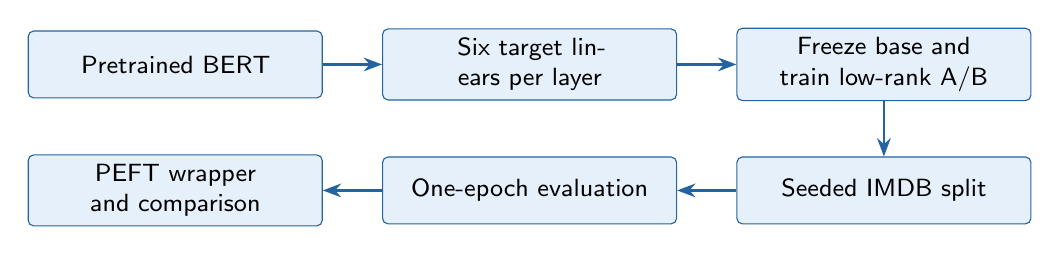
\begin{tikzpicture}[>=Stealth,stage/.style={draw=steelBlue,fill=skyBlue,rounded corners=2pt,align=center,text width=3.5cm,minimum height=.85cm,font=\small\sffamily}]
\node[stage] (a) at (0cm,0cm) {Pretrained BERT};
\node[stage] (b) at (4.5cm,0cm) {Six target linears per layer};
\node[stage] (c) at (9cm,0cm) {Freeze base and train low-rank A/B};
\node[stage] (d) at (9cm,-1.6cm) {Seeded IMDB split};
\node[stage] (e) at (4.5cm,-1.6cm) {One-epoch evaluation};
\node[stage] (f) at (0cm,-1.6cm) {PEFT wrapper and comparison};
\draw[->,thick,steelBlue] (a) -- (b);
\draw[->,thick,steelBlue] (b) -- (c);
\draw[->,thick,steelBlue] (c) -- (d);
\draw[->,thick,steelBlue] (d) -- (e);
\draw[->,thick,steelBlue] (e) -- (f);
\end{tikzpicture}%
}
\caption{The exercise pipeline, from input to checked result.}
\end{figure}

\subsection{Build and train the manual adapter}

\smallskip
\noindent The LoRA exercise begins with PyTorch and BERT imports, a fixed seed, and an MPS availability check. This provides deterministic initialization and records the accelerator environment for the later training comparison.
\label{res:lab05-lora-0003}
% coverage-cell: LABS/lab05/text-02-LoRA.ipynb cell=3 source_sha256=4a0f92d213bdbac061973b4b78ee1ae2085ab61fc15d839d1d3ec82ef996d1c4
\begin{lstlisting}[style=studycode]
import torch
import torch.nn as nn
from transformers import BertTokenizer, BertForSequenceClassification, set_seed

set_seed(42)
torch.set_num_threads(4)
print("MPS available:", torch.backends.mps.is_available())
\end{lstlisting}
\par\smallskip
% coverage-output: LABS/lab05/text-02-LoRA.ipynb cell=3 output=0 source_sha256=4a0f92d213bdbac061973b4b78ee1ae2085ab61fc15d839d1d3ec82ef996d1c4 payload_sha256=e9e9ccbf6920ec5f6f6a788110a6feaa2223c9164dc7be2fd6db4621185964fa artifact=study_guide/execution_artifacts/lab05/lab05/text-02-LoRA_cell_0003_4a0f92d213bd_output_0.txt
\label{out:lab05-lora-0003-00}
\textit{The complete progress or warning stream is reproduced in Appendix~\ref{app:lab05-diagnostics}.}
% coverage-output: LABS/lab05/text-02-LoRA.ipynb cell=3 output=1 source_sha256=4a0f92d213bdbac061973b4b78ee1ae2085ab61fc15d839d1d3ec82ef996d1c4 payload_sha256=7ec2fec204775646acfd96df4dffe23e92a7a1224aeb03c9cfbeaa53e3110eee artifact=study_guide/execution_artifacts/lab05/lab05/text-02-LoRA_cell_0003_4a0f92d213bd_output_1.txt
\label{out:lab05-lora-0003-01}
\lstinputlisting[style=terminalOutput]{../../execution_artifacts/lab05/lab05/text-02-LoRA_cell_0003_4a0f92d213bd_output_1.txt}
MPS is available on this host. The notebook's Trainer selects the device during training; the availability message alone does not prove that a particular run used it.

\smallskip
\noindent This small reporting helper totals trainable and total parameters and expresses the trainable fraction as a percentage. We use it before and after adapter insertion to quantify the parameter savings.
\label{res:lab05-lora-0004}
% coverage-cell: LABS/lab05/text-02-LoRA.ipynb cell=4 source_sha256=08a5bd64657dd2bc5a920070c7a5debf107d29ebc4b891bd0165b7da8540deea
\begin{lstlisting}[style=studycode]
# From https://github.com/huggingface/peft/issues/41#issuecomment-1404611868
def print_trainable_parameters(model):
    """
    Prints the number of trainable parameters in the model.
    """
    trainable_params = 0
    all_param = 0
    for _, param in model.named_parameters():
        all_param += param.numel()
        if param.requires_grad:
            trainable_params += param.numel()
    print(
        f"trainable params: {trainable_params} || all params: {all_param} || trainable%: {100 * trainable_params / all_param:.2f}"
    )
\end{lstlisting}
\par\smallskip
The function produces no printed result until called on a model; it is reused for both the manual and PEFT implementations.

\smallskip
\noindent We load the uncased BERT encoder with a two-class sequence-classification head and its matching tokenizer. The pretrained encoder supplies language features; the classification head is newly initialized for sentiment labels.
\label{res:lab05-lora-0007}
% coverage-cell: LABS/lab05/text-02-LoRA.ipynb cell=7 source_sha256=06bb9ab2a6d9f8dfb456f3e64025a38ea80fde36b4f0a87de4de4dd72aec98b2
\begin{lstlisting}[style=studycode]
model_name = "bert-base-uncased"
model = BertForSequenceClassification.from_pretrained(model_name, num_labels=2)
tokenizer = BertTokenizer.from_pretrained(model_name)
\end{lstlisting}
\par\smallskip
% coverage-output: LABS/lab05/text-02-LoRA.ipynb cell=7 output=0 source_sha256=06bb9ab2a6d9f8dfb456f3e64025a38ea80fde36b4f0a87de4de4dd72aec98b2 payload_sha256=df6549b17a599ed32fccb315b95da8510d5deef9e222a6e8dbe3b2757f6688b9 artifact=study_guide/execution_artifacts/lab05/lab05/text-02-LoRA_cell_0007_06bb9ab2a6d9_output_0.txt
\label{out:lab05-lora-0007-00}
\lstinputlisting[style=terminalOutput]{../../execution_artifacts/lab05/lab05/text-02-LoRA_cell_0007_06bb9ab2a6d9_output_0.txt}
Transformers warns that the classifier weights are random and must be trained for the task. The head's trainability later becomes an important difference between the manual and PEFT runs.

\smallskip
\noindent Before modifying BERT, the helper establishes the full fine-tuning baseline: every parameter in the encoder and classifier is trainable.
\label{res:lab05-lora-0008}
% coverage-cell: LABS/lab05/text-02-LoRA.ipynb cell=8 source_sha256=d1e9cdfe5bf69f65e5d02083904883e892776f67fa57efd2573d6e6e0725c2d2
\begin{lstlisting}[style=studycode]
print_trainable_parameters(model)
\end{lstlisting}
\par\smallskip
% coverage-output: LABS/lab05/text-02-LoRA.ipynb cell=8 output=0 source_sha256=d1e9cdfe5bf69f65e5d02083904883e892776f67fa57efd2573d6e6e0725c2d2 payload_sha256=bcdfc634d7cab814d85228843a2c4e3625f281c762c59310c7e1ecac663c8057 artifact=study_guide/execution_artifacts/lab05/lab05/text-02-LoRA_cell_0008_d1e9cdfe5bf6_output_0.txt
\label{out:lab05-lora-0008-00}
\lstinputlisting[style=terminalOutput]{../../execution_artifacts/lab05/lab05/text-02-LoRA_cell_0008_d1e9cdfe5bf6_output_0.txt}
All 109,483,778 parameters are initially trainable. This count is compared with the much smaller adapter-only parameter set.

\smallskip
\noindent The manual adapter wraps a linear layer with its original operation plus a rank-eight update $(xA)B$. The standard initialization uses Kaiming-uniform A and zero B, so the adapter initially contributes exactly zero while its parameters can learn.
\label{res:lab05-lora-0010}
% coverage-cell: LABS/lab05/text-02-LoRA.ipynb cell=10 source_sha256=0cce5b7e8ce3c86e6e2b800cbff4f525cff119ebd3e74a0ca004779e7d9fa56c
\begin{lstlisting}[style=studycode]
class LoRA(nn.Module):
    def __init__(self, original_layer, rank=8):
        super(LoRA, self).__init__()
        self.original_layer = original_layer
        self.rank = rank
        self.in_features = original_layer.in_features
        self.out_features = original_layer.out_features

        # Match the standard LoRA initialization: A uses Kaiming uniform, B starts at zero.
        # Transposing A for initialization gives Kaiming's fan-in the input dimension.
        self.A = nn.Parameter(torch.empty(self.in_features, rank))
        nn.init.kaiming_uniform_(self.A.T, a=5 ** 0.5)
        self.B = nn.Parameter(torch.zeros(rank, self.out_features))

    def forward(self, x):
        # The output is the original layer output plus the low-rank adaptation

        # LoRA output
        lora_output = (x @ self.A) @ self.B

        # layer output, which combines the original output with the LoRA one 
        return self.original_layer(x) + lora_output
\end{lstlisting}
\par\smallskip
This class preserves the base projection and adds a low-rank trainable path. Its parameter dimensions are input-by-rank and rank-by-output, so the added count is proportional to rank rather than input times output.

\smallskip
\noindent Each BERT encoder block has six linear projections selected here: query, key, value, attention output, and the two feed-forward transformations. Replacing them applies the same adapter construction throughout the encoder.
\label{res:lab05-lora-0012}
% coverage-cell: LABS/lab05/text-02-LoRA.ipynb cell=12 source_sha256=874659a35c7f990db050fe16bccddc5599f89de4373e4e9338b4392b04096c7e
\begin{lstlisting}[style=studycode]
for layer in model.bert.encoder.layer:
    layer.attention.self.query = LoRA(layer.attention.self.query)
    layer.attention.self.key = LoRA(layer.attention.self.key)
    layer.attention.self.value = LoRA(layer.attention.self.value)
    layer.attention.output.dense = LoRA(layer.attention.output.dense)
    layer.intermediate.dense = LoRA(layer.intermediate.dense)
    layer.output.dense = LoRA(layer.output.dense)
\end{lstlisting}
\par\smallskip
The model now contains a base projection plus a low-rank path at each selected site. Layer normalization, embeddings, and the task classifier are not replaced by this loop.

\smallskip
\noindent To make the experiment parameter-efficient, all model parameters are frozen first. The loop then enables gradients only for each manually inserted A and B matrix.
\label{res:lab05-lora-0014}
% coverage-cell: LABS/lab05/text-02-LoRA.ipynb cell=14 source_sha256=e34aa8de27b8f6cb74166cafe6d77afdceedcdb3adb1903c11beed12ce55e7a8
\begin{lstlisting}[style=studycode]
# Freeze all parameters except the LoRA parameters

# Freeze all parameters
for param in model.parameters():
    param.requires_grad = False 
    
# Unfreeze only LoRA parameters
for layer in model.modules():
    if isinstance(layer, LoRA):
        layer.A.requires_grad = True
        layer.B.requires_grad = True
\end{lstlisting}
\par\smallskip
This policy trains the adapters while leaving the pretrained encoder and the randomly initialized classifier frozen. That frozen classifier is a limitation when comparing accuracy with PEFT, which also trains its task head.

\smallskip
\noindent The parameter helper now checks whether freezing and replacement produced the expected trainable count. The assertion guards the architecture calculation against a missed or duplicated projection.
\label{res:lab05-lora-0016}
% coverage-cell: LABS/lab05/text-02-LoRA.ipynb cell=16 source_sha256=8d2681065ff9c607a7e121b2fa58b471afac57c9e1c0cbc17c669b7954e18dcf
\begin{lstlisting}[style=studycode]
print_trainable_parameters(model)
assert sum(p.numel() for p in model.parameters() if p.requires_grad) == 1_327_104
\end{lstlisting}
\par\smallskip
% coverage-output: LABS/lab05/text-02-LoRA.ipynb cell=16 output=0 source_sha256=8d2681065ff9c607a7e121b2fa58b471afac57c9e1c0cbc17c669b7954e18dcf payload_sha256=fcf4a70ef28ffe7d38ebaad6f9061493d9fd9d0262e62354525b05012ebbe070 artifact=study_guide/execution_artifacts/lab05/lab05/text-02-LoRA_cell_0016_8d2681065ff9_output_0.txt
\label{out:lab05-lora-0016-00}
\lstinputlisting[style=terminalOutput]{../../execution_artifacts/lab05/lab05/text-02-LoRA_cell_0016_8d2681065ff9_output_0.txt}
The six adapter sites across twelve layers contain 1,327,104 trainable parameters, about 1.20% of the full model. The classifier remains frozen in this manual path.

\smallskip
\noindent The IMDB dataset is shuffled with seed 42 and reduced to 2,000 training and 1,000 test examples. This small, disjoint sample keeps the demonstration manageable while preserving a reproducible comparison set.
\label{res:lab05-lora-0018}
% coverage-cell: LABS/lab05/text-02-LoRA.ipynb cell=18 source_sha256=01370b312d1c2ab4df81a516c617011c341056b58e2bb3a536ee5df65447657e
\begin{lstlisting}[style=studycode]
from datasets import load_dataset

# Load a sentiment analysis dataset
dataset = load_dataset('imdb')
train_dataset = dataset['train'].shuffle(seed=42).select(range(2000))
test_dataset = dataset['test'].shuffle(seed=42).select(range(1000))
\end{lstlisting}
\par\smallskip
% coverage-output: LABS/lab05/text-02-LoRA.ipynb cell=18 output=0 source_sha256=01370b312d1c2ab4df81a516c617011c341056b58e2bb3a536ee5df65447657e payload_sha256=b94e0cd9fbc8c9e883d1b5dad1a5e21af1d0852a9c5cd213c5aedb1ac1eb3d58 artifact=study_guide/execution_artifacts/lab05/lab05/text-02-LoRA_cell_0018_01370b312d1c_output_0.txt
\label{out:lab05-lora-0018-00}
\lstinputlisting[style=terminalOutput]{../../execution_artifacts/lab05/lab05/text-02-LoRA_cell_0018_01370b312d1c_output_0.txt}
% coverage-output: LABS/lab05/text-02-LoRA.ipynb cell=18 output=1 source_sha256=01370b312d1c2ab4df81a516c617011c341056b58e2bb3a536ee5df65447657e payload_sha256=6fc73a4b08e37dd4ea25d4722cf38be9a7b9088baaba354f347a3f9d55e6ec84 artifact=study_guide/execution_artifacts/lab05/lab05/text-02-LoRA_cell_0018_01370b312d1c_output_1.txt
\label{out:lab05-lora-0018-01}
\lstinputlisting[style=terminalOutput]{../../execution_artifacts/lab05/lab05/text-02-LoRA_cell_0018_01370b312d1c_output_1.txt}
The cached dataset is used in offline mode. The same selected rows feed both adapter implementations.

\smallskip
\noindent This metric callback converts the Trainer's logits to class predictions and computes accuracy against the reference labels. It is reused for initial evaluation, periodic validation, and final comparison.
\label{res:lab05-lora-0019}
% coverage-cell: LABS/lab05/text-02-LoRA.ipynb cell=19 source_sha256=b1cc69dce7358f1fe538d859cf4dc542bbe1c076d574afc0bdf090d01670d8b0
\begin{lstlisting}[style=studycode]
from sklearn.metrics import accuracy_score

# Function to compute accuracy
def compute_metrics(pred):
    labels = pred.label_ids
    preds = pred.predictions.argmax(-1)
    accuracy = accuracy_score(labels, preds)
    return {"accuracy": accuracy}
\end{lstlisting}
\par\smallskip
The callback returns a single accuracy metric for each evaluation event, keeping the comparison focused on held-out classification accuracy.

\smallskip
\noindent The tokenizer converts the review text into padded, truncated BERT inputs. Mapping both splits in batches prepares model-ready data once for both training approaches.
\label{res:lab05-lora-0020}
% coverage-cell: LABS/lab05/text-02-LoRA.ipynb cell=20 source_sha256=93020f6ffe151bae1ee4268d7d11778efdd31cefcde17d882cccd5049d949958
\begin{lstlisting}[style=studycode]
# Tokenize the dataset
def tokenize_function(sample):
    return tokenizer(sample['text'], padding="max_length", truncation=True)

train_dataset = train_dataset.map(tokenize_function, batched=True)
test_dataset = test_dataset.map(tokenize_function, batched=True)
\end{lstlisting}
\par\smallskip
The tokenized datasets contain aligned input IDs, attention masks, and labels; later Trainers can reuse them without retokenizing.

\smallskip
\noindent The Trainer configuration keeps an effective batch of 32 using microbatches of four and eight accumulation steps. It specifies one epoch, the shared learning rate and weight decay, evaluation and logging every ten updates, and disables external reporting.
\label{res:lab05-lora-0021}
% coverage-cell: LABS/lab05/text-02-LoRA.ipynb cell=21 source_sha256=7d8849387903055cc551113722e7ec1fa4514bc2a49d44ebee1668e2b2451d8d
\begin{lstlisting}[style=studycode]
from transformers import Trainer, TrainingArguments

batch_size = 32
num_train_epochs = 1

learning_rate = 2e-4
weight_decay = 0.01

# Define training arguments
training_args = TrainingArguments(
    output_dir='./results',
    eval_strategy="steps",
    eval_steps=10,
    learning_rate=learning_rate,
    # Accumulate smaller microbatches to retain effective batch size 32.
    per_device_train_batch_size=4,
    gradient_accumulation_steps=batch_size // 4,
    per_device_eval_batch_size=8,
    num_train_epochs=num_train_epochs,
    weight_decay=weight_decay,
    logging_dir='./logs',  # Directory for storing logs
    logging_steps=10,  # Log every 10 steps
    report_to="none",
    seed=42,
    dataloader_pin_memory=torch.cuda.is_available(),
)

# Initialize the Trainer object
trainer = Trainer(
    model=model,
    args=training_args,
    train_dataset=train_dataset,
    eval_dataset=test_dataset,
    compute_metrics=compute_metrics
)
\end{lstlisting}
\par\smallskip
The same arguments and metric callback are reused for both implementations. This cell creates the training controller but does not yet evaluate or update the model.

\smallskip
\noindent Before training, we measure the manual adapter model on the held-out split. This establishes the starting accuracy of the frozen random classifier plus untrained adapters.
\label{res:lab05-lora-0022}
% coverage-cell: LABS/lab05/text-02-LoRA.ipynb cell=22 source_sha256=885876575d5ec172025ca598be7a53b5fe4c2649d7f654a91a6fbb29531b13b0
\begin{lstlisting}[style=studycode]
# Evaluate the model
results = trainer.evaluate()
print(f"Accuracy on the validation set: {results['eval_accuracy']:.4f}")
\end{lstlisting}
\par\smallskip
% coverage-output: LABS/lab05/text-02-LoRA.ipynb cell=22 output=0 source_sha256=885876575d5ec172025ca598be7a53b5fe4c2649d7f654a91a6fbb29531b13b0 payload_sha256=fa714bdc19679c3cf97c23bd0d1d26738f1203c473a19281356ce48b7c94b803 artifact=study_guide/execution_artifacts/lab05/lab05/text-02-LoRA_cell_0022_885876575d5e_output_0.txt
\label{out:lab05-lora-0022-00}
\textit{The complete progress or warning stream is reproduced in Appendix~\ref{app:lab05-diagnostics}.}
% coverage-output: LABS/lab05/text-02-LoRA.ipynb cell=22 output=1 source_sha256=885876575d5ec172025ca598be7a53b5fe4c2649d7f654a91a6fbb29531b13b0 payload_sha256=1acb17b94ec6c013151e9bdd654bfd9f4b8d39cb3ff25c38338ba3bcfc649082 artifact=study_guide/execution_artifacts/lab05/lab05/text-02-LoRA_cell_0022_885876575d5e_output_1.txt
\label{out:lab05-lora-0022-01}
\lstinputlisting[style=terminalOutput]{../../execution_artifacts/lab05/lab05/text-02-LoRA_cell_0022_885876575d5e_output_1.txt}
Initial accuracy is 0.5070, close to chance for two balanced classes. The progress trace is retained in the diagnostics appendix.

\smallskip
\noindent The manual adapters are trained for one epoch on the seeded 2,000-review subset, with held-out evaluation at regular update intervals. The complete validation table shows how accuracy and loss change during adaptation.
\label{res:lab05-lora-0023}
% coverage-cell: LABS/lab05/text-02-LoRA.ipynb cell=23 source_sha256=dbb6eab86ae5240fa958245aa64c194ce49903e7b474cea74524fbc3adf03e5d
\begin{lstlisting}[style=studycode]
results = trainer.train()
\end{lstlisting}
\par\smallskip
% coverage-output: LABS/lab05/text-02-LoRA.ipynb cell=23 output=0 source_sha256=dbb6eab86ae5240fa958245aa64c194ce49903e7b474cea74524fbc3adf03e5d payload_sha256=96d9db66bf053cc641e4c77e8e674f469efaec422fb489d5b79a628f2ac58a64 artifact=study_guide/execution_artifacts/lab05/lab05/text-02-LoRA_cell_0023_dbb6eab86ae5_output_0.txt
\label{out:lab05-lora-0023-00}
\lstinputlisting[style=terminalOutput]{../../execution_artifacts/lab05/lab05/text-02-LoRA_cell_0023_dbb6eab86ae5_output_0.txt}
The 62-update run reports the per-checkpoint losses and accuracies in full. Its training time is about 810 seconds on this host; the assigned classifier remains frozen, so interpret this result as the notebook's adapter-only implementation rather than a fully matched classifier fine-tune.

\smallskip
\noindent After the manual adapter epoch, the same held-out set is evaluated again to quantify its endpoint under the shared metric.
\label{res:lab05-lora-0024}
% coverage-cell: LABS/lab05/text-02-LoRA.ipynb cell=24 source_sha256=885876575d5ec172025ca598be7a53b5fe4c2649d7f654a91a6fbb29531b13b0
\begin{lstlisting}[style=studycode]
# Evaluate the model
results = trainer.evaluate()
print(f"Accuracy on the validation set: {results['eval_accuracy']:.4f}")
\end{lstlisting}
\par\smallskip
% coverage-output: LABS/lab05/text-02-LoRA.ipynb cell=24 output=0 source_sha256=885876575d5ec172025ca598be7a53b5fe4c2649d7f654a91a6fbb29531b13b0 payload_sha256=877c38d7ab46c5abc348289e855ced8f45bb11506a79830fbbf7c6e874c7ede9 artifact=study_guide/execution_artifacts/lab05/lab05/text-02-LoRA_cell_0024_885876575d5e_output_0.txt
\label{out:lab05-lora-0024-00}
\textit{The complete progress or warning stream is reproduced in Appendix~\ref{app:lab05-diagnostics}.}
% coverage-output: LABS/lab05/text-02-LoRA.ipynb cell=24 output=1 source_sha256=885876575d5ec172025ca598be7a53b5fe4c2649d7f654a91a6fbb29531b13b0 payload_sha256=fd2e0ad8ecc921054169332e08eb993c249220e333c68c31eca34fd0e79079a7 artifact=study_guide/execution_artifacts/lab05/lab05/text-02-LoRA_cell_0024_885876575d5e_output_1.txt
\label{out:lab05-lora-0024-01}
\lstinputlisting[style=terminalOutput]{../../execution_artifacts/lab05/lab05/text-02-LoRA_cell_0024_885876575d5e_output_1.txt}
Accuracy rises from 0.5070 to 0.6580. This is an observed result on 1,000 selected reviews and the fixed random classifier, not a general benchmark.

\subsection{Apply the same encoder adapters with PEFT}

The PEFT path starts from a freshly loaded BERT checkpoint after the manual model is released. Its target-module list is derived from the same six encoder linears per layer. The library also keeps the sequence-classification head trainable; this adds 1,538 parameters and means the final accuracy comparison is informative but not perfectly controlled.

\smallskip
\noindent Before testing PEFT, the notebook releases the manual Trainer and model, clears cached MPS allocations, resets the seed, and reloads a fresh BERT classifier. This prevents learned weights from leaking into the second approach.
\label{res:lab05-lora-0027}
% coverage-cell: LABS/lab05/text-02-LoRA.ipynb cell=27 source_sha256=7bd0791787a21da125e8490e2208d325e79b15ad93db6883f06949789b6e2785
\begin{lstlisting}[style=studycode]
# Release the manually adapted model/trainer before loading a fresh baseline.
import gc
globals().pop("trainer", None)
globals().pop("model", None)
gc.collect()
if torch.backends.mps.is_available():
    torch.mps.empty_cache()

set_seed(42)
model_name = "bert-base-uncased"
model = BertForSequenceClassification.from_pretrained(model_name)
tokenizer = BertTokenizer.from_pretrained(model_name)
\end{lstlisting}
\par\smallskip
% coverage-output: LABS/lab05/text-02-LoRA.ipynb cell=27 output=0 source_sha256=7bd0791787a21da125e8490e2208d325e79b15ad93db6883f06949789b6e2785 payload_sha256=df6549b17a599ed32fccb315b95da8510d5deef9e222a6e8dbe3b2757f6688b9 artifact=study_guide/execution_artifacts/lab05/lab05/text-02-LoRA_cell_0027_7bd0791787a2_output_0.txt
\label{out:lab05-lora-0027-00}
\lstinputlisting[style=terminalOutput]{../../execution_artifacts/lab05/lab05/text-02-LoRA_cell_0027_7bd0791787a2_output_0.txt}
The warning again identifies the newly initialized classification head. Reloading it under the same seed makes the PEFT branch start from a reproducible baseline.

\smallskip
\noindent PEFT's LoRA configuration uses rank eight, alpha 32, dropout 0.1, and targets the same six encoder Linear projections per layer. Its sequence-classification wrapper also keeps the task head trainable.
\label{res:lab05-lora-0029}
% coverage-cell: LABS/lab05/text-02-LoRA.ipynb cell=29 source_sha256=882cbe44477848b502e19ef82ffb5cffb370c5755343a64b743032232d6a41e4
\begin{lstlisting}[style=studycode]
from peft import LoraConfig, get_peft_model, PeftModelForSequenceClassification

config = LoraConfig(
    r=8,
    lora_alpha=32, 
    lora_dropout=0.1,
    bias="none",
    # Select the same six linear transformations in each encoder block.
    target_modules=[
        name for name, module in model.named_modules()
        if name.startswith("bert.encoder.layer.") and isinstance(module, nn.Linear)
    ],
)

peft_model = PeftModelForSequenceClassification(model, peft_config=config)
\end{lstlisting}
\par\smallskip
The PEFT model now contains low-rank modules at the selected sites. Its trainable count will include the classification head as well as the adapters.

\smallskip
\noindent This type inspection confirms that \texttt{get\_peft\_model} returned the sequence-classification PEFT wrapper expected for the task.
\label{res:lab05-lora-0030}
% coverage-cell: LABS/lab05/text-02-LoRA.ipynb cell=30 source_sha256=9ff926a47cc4ee6d276c5924e17430173ce49c2da5ab80950dc783a2d9a7e831
\begin{lstlisting}[style=studycode]
type(peft_model)
\end{lstlisting}
\par\smallskip
% coverage-output: LABS/lab05/text-02-LoRA.ipynb cell=30 output=0 source_sha256=9ff926a47cc4ee6d276c5924e17430173ce49c2da5ab80950dc783a2d9a7e831 payload_sha256=f49d968a241f40a6e68dc374631cc5b273546fa6d38d641bf2dfb7d613842dc9 artifact=study_guide/execution_artifacts/lab05/lab05/text-02-LoRA_cell_0030_9ff926a47cc4_output_0.txt
\label{out:lab05-lora-0030-00}
\lstinputlisting[style=terminalOutput]{../../execution_artifacts/lab05/lab05/text-02-LoRA_cell_0030_9ff926a47cc4_output_0.txt}
The Python type is `PeftModelForSequenceClassification`, so the task-specific classifier is preserved by the wrapper.

\smallskip
\noindent Printing the first encoder block verifies where PEFT inserted its A and B projections and shows that the original linear layers remain as the adapter base.
\label{res:lab05-lora-0032}
% coverage-cell: LABS/lab05/text-02-LoRA.ipynb cell=32 source_sha256=9c035399ab5f1a2c41c7d5b06a05c10bd97585f9bdb718ba1f7af03aca4a8d03
\begin{lstlisting}[style=studycode]
peft_model.bert.encoder.layer[0]
\end{lstlisting}
\par\smallskip
% coverage-output: LABS/lab05/text-02-LoRA.ipynb cell=32 output=0 source_sha256=9c035399ab5f1a2c41c7d5b06a05c10bd97585f9bdb718ba1f7af03aca4a8d03 payload_sha256=c56b1b8303d46217a80fc59108b5c1407f45b0c6cac87efae9eca6a9d481b61c artifact=study_guide/execution_artifacts/lab05/lab05/text-02-LoRA_cell_0032_9c035399ab5f_output_0.txt
\label{out:lab05-lora-0032-00}
\lstinputlisting[style=terminalOutput]{../../execution_artifacts/lab05/lab05/text-02-LoRA_cell_0032_9c035399ab5f_output_0.txt}
The module tree displays adapters on the attention and feed-forward linears. This is the library-managed counterpart to the manual replacements above.

\smallskip
\noindent The PEFT helper calculates trainable parameters after wrapping. Comparing the result with the manual count reveals whether the task head is included.
\label{res:lab05-lora-0034}
% coverage-cell: LABS/lab05/text-02-LoRA.ipynb cell=34 source_sha256=8622472c22954188c6e70551ec322752bcb1b07cf3c2b9439efe1e8b82c355ed
\begin{lstlisting}[style=studycode]
peft_model.print_trainable_parameters()
\end{lstlisting}
\par\smallskip
% coverage-output: LABS/lab05/text-02-LoRA.ipynb cell=34 output=0 source_sha256=8622472c22954188c6e70551ec322752bcb1b07cf3c2b9439efe1e8b82c355ed payload_sha256=dfd1f93987a817cebdaa8abee80dd06cd57db2873a1b26a83bde2d0bf4d635e9 artifact=study_guide/execution_artifacts/lab05/lab05/text-02-LoRA_cell_0034_8622472c2295_output_0.txt
\label{out:lab05-lora-0034-00}
\lstinputlisting[style=terminalOutput]{../../execution_artifacts/lab05/lab05/text-02-LoRA_cell_0034_8622472c2295_output_0.txt}
PEFT trains 1,328,642 parameters, including 1,538 classifier weights and biases, versus 1,327,104 manual adapter parameters. The accuracy comparison therefore is not perfectly controlled.

\smallskip
\noindent A second Trainer is constructed with the same tokenized splits, metric callback, and training arguments. Only the model object changes to the PEFT-wrapped classifier.
\label{res:lab05-lora-0036}
% coverage-cell: LABS/lab05/text-02-LoRA.ipynb cell=36 source_sha256=e5822d2c0f6d83063dd90a397b028f7796226a3e82b90aeeffe5a01d406dbccf
\begin{lstlisting}[style=studycode]
from transformers import Trainer, TrainingArguments

# Initialize the Trainer object
trainer = Trainer(
    model=peft_model,
    args=training_args, # we will recycle the same training arguments as before!
    train_dataset=train_dataset, # also datasets, 
    eval_dataset=test_dataset,
    compute_metrics=compute_metrics # and compute_metrics
)
\end{lstlisting}
\par\smallskip
The comparison is ready to run with the same one-epoch schedule and effective batch size as the manual path.

\smallskip
\noindent PEFT adapters are trained for one epoch using the shared Trainer configuration. The saved table records validation loss and accuracy at each logged checkpoint.
\label{res:lab05-lora-0037}
% coverage-cell: LABS/lab05/text-02-LoRA.ipynb cell=37 source_sha256=a2c3063cd5a534cfca2e804c13bc1931abfb77a8aab492c6ab2507ecdb8de9a1
\begin{lstlisting}[style=studycode]
trainer.train()
\end{lstlisting}
\par\smallskip
% coverage-output: LABS/lab05/text-02-LoRA.ipynb cell=37 output=0 source_sha256=a2c3063cd5a534cfca2e804c13bc1931abfb77a8aab492c6ab2507ecdb8de9a1 payload_sha256=ce039b4bc87a8982dff916717096804e8acbf60089252bd79c28fcbfe79949aa artifact=study_guide/execution_artifacts/lab05/lab05/text-02-LoRA_cell_0037_a2c3063cd5a5_output_0.txt
\label{out:lab05-lora-0037-00}
\lstinputlisting[style=terminalOutput]{../../execution_artifacts/lab05/lab05/text-02-LoRA_cell_0037_a2c3063cd5a5_output_0.txt}
% coverage-output: LABS/lab05/text-02-LoRA.ipynb cell=37 output=1 source_sha256=a2c3063cd5a534cfca2e804c13bc1931abfb77a8aab492c6ab2507ecdb8de9a1 payload_sha256=358fb9371e16926cfd56936e8f74360e712f75717653133f5d2d005de942056b artifact=study_guide/execution_artifacts/lab05/lab05/text-02-LoRA_cell_0037_a2c3063cd5a5_output_1.txt
\label{out:lab05-lora-0037-01}
\lstinputlisting[style=terminalOutput]{../../execution_artifacts/lab05/lab05/text-02-LoRA_cell_0037_a2c3063cd5a5_output_1.txt}
The 62-update run reports training loss 0.5761 and runtime 814.4 seconds; the full step table is preserved. The task head is trainable here, unlike in the manual branch, so the accuracy difference combines implementation and head-training effects.

\smallskip
\noindent The final cell evaluates the trained PEFT classifier once more on the held-out reviews so its endpoint can be read alongside the manual result.
\label{res:lab05-lora-0038}
% coverage-cell: LABS/lab05/text-02-LoRA.ipynb cell=38 source_sha256=885876575d5ec172025ca598be7a53b5fe4c2649d7f654a91a6fbb29531b13b0
\begin{lstlisting}[style=studycode]
# Evaluate the model
results = trainer.evaluate()
print(f"Accuracy on the validation set: {results['eval_accuracy']:.4f}")
\end{lstlisting}
\par\smallskip
% coverage-output: LABS/lab05/text-02-LoRA.ipynb cell=38 output=0 source_sha256=885876575d5ec172025ca598be7a53b5fe4c2649d7f654a91a6fbb29531b13b0 payload_sha256=96c36cefdb3a5d314bd965a9af2e27247c96df29c2578a21ccedabf01b7855d9 artifact=study_guide/execution_artifacts/lab05/lab05/text-02-LoRA_cell_0038_885876575d5e_output_0.txt
\label{out:lab05-lora-0038-00}
\textit{The complete progress or warning stream is reproduced in Appendix~\ref{app:lab05-diagnostics}.}
% coverage-output: LABS/lab05/text-02-LoRA.ipynb cell=38 output=1 source_sha256=885876575d5ec172025ca598be7a53b5fe4c2649d7f654a91a6fbb29531b13b0 payload_sha256=26d8be7a0e0e185e5e38a86dab7986333de62b9c53f283172c4ac8d0966795a2 artifact=study_guide/execution_artifacts/lab05/lab05/text-02-LoRA_cell_0038_885876575d5e_output_1.txt
\label{out:lab05-lora-0038-01}
\lstinputlisting[style=terminalOutput]{../../execution_artifacts/lab05/lab05/text-02-LoRA_cell_0038_885876575d5e_output_1.txt}
Final accuracy is 0.8170 on this selected test subset. The difference from the manual 0.6580 result is suggestive for this run, but the two branches differ in classifier trainability and PEFT dropout.

\clearpage

\appendix

\section{Diagnostic output and earlier authentication attempt}

\label{app:lab05-diagnostics}

The complete warnings and progress-only streams omitted from the computational narrative are retained here. They remain tied to their source outputs by the coverage manifest and raw payload hashes.

\paragraph{Diagnostic stream from text-01-quantization.ipynb, cell 39.}

\lstinputlisting[style=terminalOutput]{../../execution_artifacts/lab05/lab05/text-01-quantization_cell_0039_ecb57f6ce8cd_output_0.txt}

\paragraph{Diagnostic stream from text-02-LoRA.ipynb, cell 3.}

\lstinputlisting[style=terminalOutput]{../../execution_artifacts/lab05/lab05/text-02-LoRA_cell_0003_4a0f92d213bd_output_0.txt}

\paragraph{Diagnostic stream from text-02-LoRA.ipynb, cell 22.}

\lstinputlisting[style=terminalOutput]{../../execution_artifacts/lab05/lab05/text-02-LoRA_cell_0022_885876575d5e_output_0.txt}

\paragraph{Diagnostic stream from text-02-LoRA.ipynb, cell 24.}

\lstinputlisting[style=terminalOutput]{../../execution_artifacts/lab05/lab05/text-02-LoRA_cell_0024_885876575d5e_output_0.txt}

\paragraph{Diagnostic stream from text-02-LoRA.ipynb, cell 38.}

\lstinputlisting[style=terminalOutput]{../../execution_artifacts/lab05/lab05/text-02-LoRA_cell_0038_885876575d5e_output_0.txt}

\paragraph{Earlier authentication failure.} The first saved attempt stopped at the notebook's local Hugging Face authentication check. The later execution used the account's existing credential store and successfully loaded the approved checkpoint. No credential value is included here.

\begin{lstlisting}[style=terminalOutput]

RuntimeError: Llama 3.2 requires an approved Hugging Face account. Run hf auth login locally or set HF_TOKEN, then rerun.

\end{lstlisting}

\section{Execution and reproducibility notes}

No Lab05 lecture recording was available among the supplied course files. The only additional Whisper item inspected was a computer-vision lecture on object detection and segmentation, so it was excluded as unrelated. The professor's promised Laboratory 05 recording can be incorporated later. Explanations and numerical claims here follow the notebook source and its recorded executions rather than inferred lecture content.

The quantization arithmetic uses seeded toy tensors. The Llama comparison uses checkpoint revisions and exact package versions recorded in \path{lab05/execution/environment.json}; CPU timing depends on the host, thread scheduling, backend, and model-cache state. Serialized state size is not peak inference memory. The LoRA runs use a seeded 2,000/1,000 IMDB subset, microbatch four, eight-step accumulation, and one epoch. Manual training took about 810 seconds and PEFT about 814 seconds on this host. The manual path freezes the new classification head, while PEFT trains it, so the 0.658 versus 0.817 accuracy results are not an isolated causal comparison of the adapter implementations.

\end{document}

\end{document}
